%
% teil3.tex -- Beispiel-File für Teil 3
%
% (c) 2020 Prof Dr Andreas Müller, Hochschule Rapperswil
%
% !TEX root = ../../buch.tex
% !TEX encoding = UTF-8
%
\section{Gleichungen mit einer Komponente
\label{reaktdiff:section:einKomponent}}
\kopfrechts{Gleichungen mit einer Komponente}%
Die einfachste Reaktionsdiffusionsgleichung ist die, welche nur einen Stoff beschreibt.
Die Reaktionsdiffusionsgleichung ist in diesem Fall
\begin{equation*}
\label{reaktdiff:equation:fkpp}
\frac{\partial c}{\partial t} = D \frac{\partial^2 c}{\partial x^2} + rc(1-c).
\end{equation*}
Um die Komplexität zu reduzieren ist \(c\) eindimensional. 
Die Gleichung \eqref{reaktdiff:equation:fkpp} ist auch als Fisher-KPP-Gleichung \cite{reaktdiff:wikipedia_kpp_fisher} bekannt, benannt nach Roland Fisher, Andrey Kolmogorov, Ivan Petrovsky und Nikolai Piskunov.
\index{Fisher-KPP-Gleichung}%
\index{Kolmogorov, Andrey}%
\index{Fisher, Roland}%
\index{Petrovsky, Ivan}%
\index{Piskunov, Nikolai}%

\subsection{Stabilitätsanalyse mit Fourier-Theorie
\label{reaktdiff:subsection:fkppmathe}}
Aus der Gleichung können die stationären Lösungen abgeleitet werden.
\index{stationare Losung@stationäre Lösung}%
Setzten wir \(\frac{\partial c}{\partial t} = 0\) und \(\Delta c = 0\) erhalten wir die stationäre Lösung
\begin{equation}
\label{reaktdiff:equation:stationaer}
0 = rc(1-c).
\end{equation}

\subsubsection{Linearisierung}
\index{Linearisierung}%
Die Lösungen der Gleichung
\eqref{reaktdiff:equation:stationaer}
sind \(c = 0\) und \(c = 1\).
Um nun das Verhalten dieser Lösungen zu untersuchen, fügen wir eine kleine Störung \(\varepsilon\) hinzu, wobei \(\varepsilon \ll 1\).

Für den Fall \(c = 0\) erhalten wir
\begin{equation}
\label{reaktdiff:equation:störung0}
\frac{\partial \varepsilon}{\partial t} = D \frac{\partial^2 \varepsilon}{\partial x^2} + r\varepsilon(1-\varepsilon).
\end{equation}
Da \(\varepsilon\) sehr klein ist, kann man den Term \(1-\varepsilon\) durch \(1\) ersetzen.
Somit wird die Gleichung \eqref{reaktdiff:equation:störung0} zu
\begin{equation}
\label{reaktdiff:equation:störung0vereinfach}
\frac{\partial \varepsilon}{\partial t} \approx D \frac{\partial^2 \varepsilon}{\partial x^2}  + r\varepsilon.
\end{equation}
Die Gleichung \eqref{reaktdiff:equation:störung0vereinfach} ist eine lineare partielle Differentialgleichung.
Dasselbe gilt für den Fall \(c = 1\) bei welchem wir
%Für den Fall \(c = 1\) erhalten wir
\begin{equation}
\label{reaktdiff:equation:störung1}
\frac{\partial \varepsilon}{\partial t} = D \frac{\partial^2 \varepsilon}{\partial x^2} - r\varepsilon(1-\varepsilon)
\end{equation}
erhalten.
Wieder können wir den Term \(1-\varepsilon\) durch \(1\) ersetzen.
Somit wird die Gleichung \eqref{reaktdiff:equation:störung1} zu
\begin{equation}
\label{reaktdiff:equation:störung1vereinfach}
\frac{\partial \varepsilon}{\partial t} \approx D \frac{\partial^2 \varepsilon}{\partial x^2} - r\varepsilon.
\end{equation}
Die Gleichung \eqref{reaktdiff:equation:störung1vereinfach} ist ebenfalls eine lineare partielle Differentialgleichung.
Man sieht, dass der Unterschied zwischen den beiden Gleichungen \eqref{reaktdiff:equation:störung0vereinfach} und \eqref{reaktdiff:equation:störung1vereinfach} nur das Vorzeichen des \(r \varepsilon\)-Terms ist.

\subsubsection{Fourier-Ansatz}
Die stationären Lösungen hängen nicht von den Raumkoordinaten ab.
Eine allgemeine Lösung wird auch von \(x\) abhängen.
Tatsächlich beboachtet man in der Natur bei solchen Systemen oft
das Auftreten von regelmässigen oder periodischen Mustern, wie man
auch in Abbildung \ref{reaktdiff:fig:gs} und \ref{reaktdiff:fig:fhn}
sehen kann.
Wir versuchen, diesen Mustern mit einem Fourier-Ansatz Rechnung zu tragen.
\index{Fourier-Ansatz}%

Um die Gleichung zu lösen setzen wir \(\varepsilon(x,t) = c_k(t) e^{ikx}\) ein.
Die Ableitungen werden zu
\begin{align*}
\frac{\partial \varepsilon}{\partial t} &= \dot{c}_k(t) e^{ikx},\\
\frac{\partial^2 \varepsilon}{\partial x^2} &= -k^2 c_k(t) e^{ikx}.
\end{align*}
Durch Einsetzen dieser Ableitungen in die Gleichung \eqref{reaktdiff:equation:störung0vereinfach} ergibt sich
\begin{equation}
\label{reaktdiff:equation:störung0vereinfachk}
\dot{c}_k(t) e^{ikx} = -D k^2 c_k(t) e^{ikx} + r c_k(t) e^{ikx}.
\end{equation}
Teilen wir die Gleichung \eqref{reaktdiff:equation:störung0vereinfachk} durch \(e^{ikx}\) erhalten wir
\begin{equation}
\label{reaktdiff:equation:störung0vereinfachk2}
\dot{c}_k(t) = -D k^2 c_k(t) + r c_k(t).
\end{equation}
Die Gleichung \eqref{reaktdiff:equation:störung0vereinfachk2} ist eine gewöhnliche Differentialgleichung.
Die Lösung der Gleichung \eqref{reaktdiff:equation:störung0vereinfachk2} ist
\begin{equation}
\label{reaktdiff:equation:störung0vereinfachk3}
c_k(t) = c_k(0) e^{(r - D k^2)t}.
\end{equation}
Setzen wir nun die Gleichung \eqref{reaktdiff:equation:störung0vereinfachk3} in die Gleichung \eqref{reaktdiff:equation:störung1vereinfach} ein, erhalten wir
\begin{equation}
\label{reaktdiff:equation:störung1vereinfachk}
\dot{c}_k(t) = -D k^2 c_k(t) - r c_k(t).
\end{equation}
Führen wir dieselbe Rechnung wie bei der 
Gleichung \eqref{reaktdiff:equation:störung0vereinfachk2} durch, erhalten wir
\begin{equation}
\label{reaktdiff:equation:störung1vereinfachk2}
c_k(t) = c_k(0) e^{(-r - D k^2)t}.
\end{equation}
\eqref{reaktdiff:equation:störung0vereinfachk3} und \eqref{reaktdiff:equation:störung1vereinfachk2} unterscheiden sich nur durch das Vorzeichen von \(r\).

\subsubsection{Stabilität}
Aus den beiden Gleichungen \eqref{reaktdiff:equation:störung0vereinfachk3} und \eqref{reaktdiff:equation:störung1vereinfachk2} können wir die Stabilität der stationären Lösungen \(c = 0\) und \(c = 1\) ablesen.
\index{Stabilitat@Stabilität}%
Unter der Annahmen dass \(D\) und \(r\) immmer positiv sind, ist die stationäre Lösung \(c = 1\) stabil.
Die stationäre Lösung \(c = 0\) ist instabil wenn \(r-Dk^2 > 0\) und stabil wenn \(r-Dk^2 < 0\).
Somit werden kleine Störungen um \(c = 0\) wachsen, wenn \(k < \!\sqrt{\frac{r}{D}}\), und abklingen, wenn \(k > \!\sqrt{\frac{r}{D}}\).

Wie bereits erwähnt, ist eine Anwendung der Fisher-KPP-Gleichung die Ausbreitung von Populationen.
Die stationären Lösungen \(c = 0\) und \(c = 1\) entsprechen dem Fall, in dem die Population nicht existiert, bzw. dem Fall, in dem die Population ihre maximale Größe erreicht hat.
Die Stabilität der stationäre Lösungen \(c = 0\) und \(c = 1\) zeigt, dass die Population immer wachsen wird, wenn sie klein ist, und abklingen wird, wenn sie gross ist.

\subsection{Wellenlösung in einer Raumdimension
\label{reaktdiff:subsection:fkppwelle}}
Die Fisher-KPP-Gleichung in einer Dimension hat eine Wellenlösung.
Die Wellenlösung ist eine Lösung der Form
\begin{equation*}
\label{reaktdiff:equation:fkppwelle}
c(x,t) = C(z), \text{ wobei } z = x - vt,
\end{equation*}
wobei \(C\) eine Funktion ist, die die Form der Welle beschreibt und \(v\) die Geschwindigkeit der Welle ist.
Für die Lösung benötigen wir die Ableitungen
\begin{align*}
\frac{\partial c}{\partial t} &= \frac{\partial C}{\partial z}\frac{\partial z}{\partial t} = -vC'(z),
\\
\frac{\partial^2 c}{\partial x^2} &= C''(z).
\end{align*}
Setzen wir die Ableitungen in die Fisher-KPP-Gleichung \eqref{reaktdiff:equation:fkpp} ein, erhalten wir
\begin{equation*}
\label{reaktdiff:equation:fkppwelle2}
-vC'(z) = D C''(z) + rC(z)(1-C(z)).
\end{equation*}
Das ergibt die nichtlineare gewöhnliche Differentialgleichung
\begin{equation}
    \label{reaktdiff:equation:fkppwelle3}
    -vC'(z) - D C''(z) - rC(z)(1-C(z)) = 0
\end{equation}
für \(C(z)\).
Für die Analyse untersuchen wir die Gleichung \eqref{reaktdiff:equation:fkppwelle3} im Grenzfall \(C(z) \ll 1\).
Das heisst, dass \(1 - C(z)\approx 1\).
Um die Gleichung zu lösen, setzen wir \(C(z) = C(0) e^{\lambda z}\) ein.
Somit wird die Gleichung \eqref{reaktdiff:equation:fkppwelle3} zu
\begin{equation*}
D\lambda^2 + v\lambda + r = 0.
\end{equation*}
Ihre Lösung ist
\begin{equation}
\label{reaktdiff:equation:fkppwelle5}
\lambda = \frac{-v \pm \!\sqrt{v^2 - 4rD}}{2D}.
\end{equation}
Aus der Gleichung \eqref{reaktdiff:equation:fkppwelle5} ist ersichtlich, dass die Wellenlösung nur möglich ist, wenn \(v \ge 2\!\sqrt{rD}\).

\subsection{Numerische Simulation der Fisher-KPP-Gleichung
\label{reaktdiff:subsection:fkppsimulation}}
Die Visualisierung der Fisher-KPP-Gleichung ist unspektakulär.
Die Simulation in Abbildung \ref{reaktdiff:figure:fisher_kpp_simulation} zeigt eine Welle die sich mit konstanter Geschwindigkeit \(v = 2\!\sqrt{rD}\) ausbreitet.
Denoch regt die Simulation zum Nachdenken an.
Was wäre nun wenn es einen zweiten Stoff gäbe, welcher die Reaktion beeinflusst?
% besser 1D
\begin{figure}
    \centering
    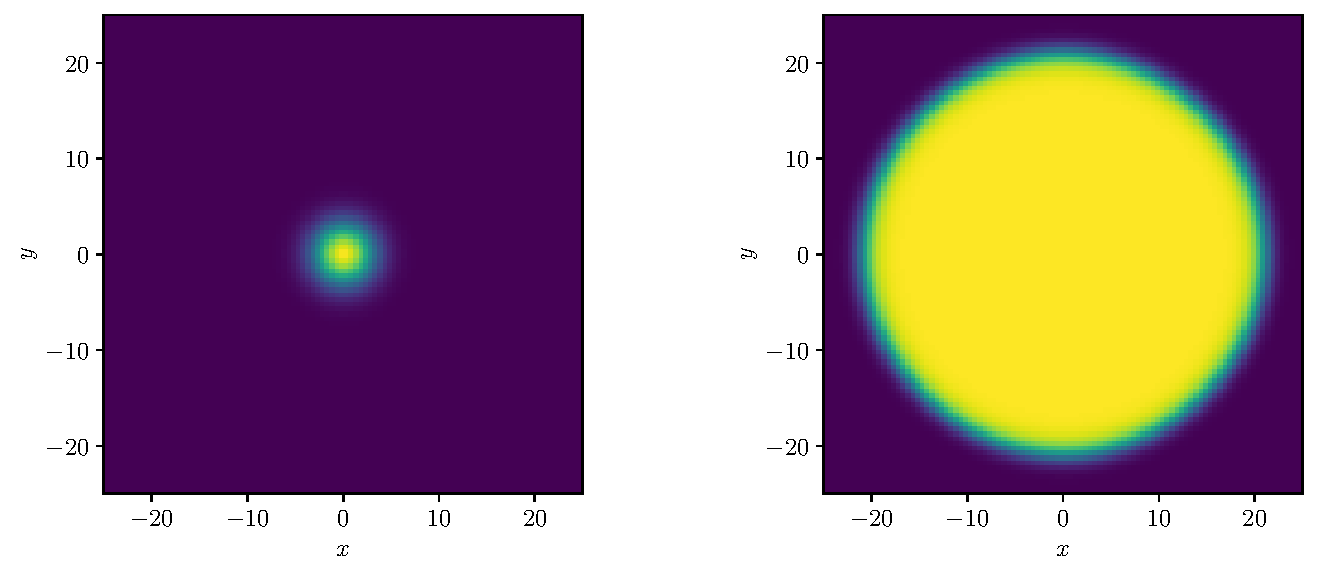
\includegraphics[width=\textwidth]{papers/reaktdiff/images/Fisher_KPP/fisher_kpp_2d_wave_comparison.pdf}
    \caption{Simulation der Fisher-KPP-Gleichung mit \(D = 0.1\) und \(r = 1\). Die Welle breitet sich mit einer Geschwindigkeit von \(v = 0.01\) aus. Das linke Bild zeigt die Simulation zum Zeitpunkt \(t = 0\) und das rechte Bild zum Zeitpunkt \(t = 25\).}
    \label{reaktdiff:figure:fisher_kpp_simulation}
\end{figure}
%
